\chapter{Μέθοδοι προσομοίωσης} \label{ch:simulation-methods}
Στο κεφάλαιο αυτό περιγράφεται η υλοποίηση του συστήματος, με βάση τη θεωρητική ανάλυση που παρουσιάστηκε στο προηγούμενο κεφάλαιο. 
Αρχικά παρουσιάζεται η πλατφόρμα και τα εργαλεία που χρησιμοποιήθηκαν.
Στη συνέχεια παρουσιάζονται όσα υλοποιήθηκαν για τη μελέτη του αντικειμένου:
\begin{itemize}
\item Η μελέτη επιρροής μεταβλητών σε έναν \en{Electron Beam Scanner}, τόσο σε θεωρητικό επίπεδο όσο και στο προσομοιωμένο μοντέλο του \en{CST}
\item Ο τρόπος προσομοίωσης ενός \en{Electron Beam Scanner} εξολοκλήρου στο \en{CST}
\item Η βελτίωση της μεθόδου προσομοίωσης, χρησιμοποιώντας το \en{CST} ως το μέσο προσομοίωσης του ηλεκτρικού πεδίου της κύριας δέσμης και στη συνέχεια το \en{MATLAB} για τον υπολογισμό των τροχιών των σωματιδίων της δέσμης ανίχνευσης μέσα στο πεδίο που εξάγεται από το \en{CST}
\end{itemize}

\section{Εργαλεία που χρησιμοποιήθηκαν}
Για την υλοποίηση των προσομοιώσεων χρησιμοποιήθηκε το πρόγραμμα \en{CST Particle Studio}, της σουίτας προγραμμάτων προσομοίωσης \en{CST Studio Suite}. 
Για την επεξεργασία και επιπλέον ανάλυση των αποτελεσμάτων του \en{CST}, καθώς και βοηθητικά για τη βελτίωση του μοντέλου στο \en{CST} χρησιμοποιήθηκε το πρόγραμμα \en{MATLAB}. 
Τα προγράμματα παρουσιάζονται πιο αναλυτικά παρακάτω.

\subsection{Το \en{CST Particle Studio}}
%\begin{figure}[tph]
%
\includegraphics[width=0.25\textwidth]{images/CST-logo}
%\centering
%\caption{Το λογότυπο του \en{CST}.}
%\label{img:CSTlogo}
%\end{figure}

Το \en{CST PARTICLE STUDIO\textsuperscript{\textregistered} (CST\textsuperscript{\textregistered} PS) } είναι ένα εξειδικευμένο εργαλείο για την γρήγορη και ακριβή ανάλυση δυναμικών για φορτισμένα σωματίδια σε τρισδιάστατα ηλεκτρομαγνητικά πεδία.
Είναι ένα ισχυρό εργαλείο, κατάλληλο για μεγάλο φάσμα εργασιών, από σχεδιασμό \en{magnetrons} και ρύθμιση σωλήνων ηλεκτρονίων έως μοντελοποίηση πηγών σωματιδίων και εξαρτημάτων για επιταχυντές.

%\en{The particle tracking solver can model the behavior of particles through static fields, and with the gun iteration, space charge limited emission. }
Ο \en{particle-in-cell (PIC) solver}, ο οποίος μπορεί να λειτουργήσει στο πεδίο του χρόνου, μπορεί να εκτελέσει μια πλήρη προσομοίωση σωματιδίων και ηλεκτρομαγνητικών πεδίων.

Για σχετικιστικές εφαρμογές, ο \en{wakefield solver} μπορεί να υπολογίσει πώς τα πεδία που δημιουργούνται από σωματίδια που κινούνται στην (ή κοντά στην) ταχύτητα του φωτός, αλληλεπιδρούν με τη δομή γύρω τους.

Το \en{CST PS} έχει ενσωματωμένα τα \en{3D EM modules} του \en{CST STUDIO SUITE\textsuperscript{\textregistered}}, όπως τα \en{CST EM STUDIO\textsuperscript{\textregistered} electro-} και \en{magnetostatic solvers} και το \en{CST MICROWAVE STUDIO\textsuperscript{\textregistered} eigenmode solver}.

Είναι πλήρως ενσωματωμένα στο περιβάλλον σχεδίασης \en{CST STUDIO SUITE}, χρησιμοποιώντας έτσι τις δυνατότητες μοντελοποίησης και τα \en{import interfaces}.

Το \en{CST PS} βασίζεται στη γνώση, την έρευνα και την ανάπτυξη των αλγορίθμων που χρησιμοποιήθηκαν στο πακέτο προσομοίωσης \en{MAFIA-4}. 
Ο \en{PIC solver} μπορεί επίσης να εκμεταλλευτεί δυνατότητες \en{GPU computing}, προσφέροντας σημαντικές βελτιώσεις στην απόδοση, σε συμβατό υλικό.

\subsection{Το \en{MATLAB}}
Το \en{MATLAB (MATrix LABoratory)} είναι ένα περιβάλλον αριθμητικής υπολογιστικής και μια προγραμματιστική γλώσσα τέταρτης γενιάς. 
Το \en{MATLAB} δίνει έχει δυνατότητες όπως αποτελεσματικό πολλαπλασιασμό πινάκων, γραφική παράσταση συναρτήσεων και δεδομένων, υλοποίηση αλγορίθμων, δημιουργία \en{user interfaces} και δυνατότητα διεπαφής με προγράμματα γραμμένα σε άλλες γλώσσες, όπως
\en{C, C\nolinebreak\hspace{-.05em}\raisebox{.4ex}{\tiny\bf +}\nolinebreak\hspace{-.10em}\raisebox{.4ex}{\tiny\bf +}, C$\sharp$, Java, Fortran} και \en{Python}.

Αν και το \en{MATLAB} προορίζεται κυρίως για αριθμητικούς υπολογισμούς, έχει προαιρετικό \en{toolbox} που χρησιμοποιεί τη συμβολική μηχανή \en{MuPAD}, επιτρέποντας έτσι την εκτέλεση συμβολικών υπολογισμών.
Ένα επιπλέον πακέτο, το \en{Simulink}, προσθέτει δυνατότητα προσομοιώσεων σε διάφορους τομείς και δυνατότητες μοντελοποίησης για δυναμικά και ενσωματωμένα συστήματα.

%\begin{figure}[tph]
%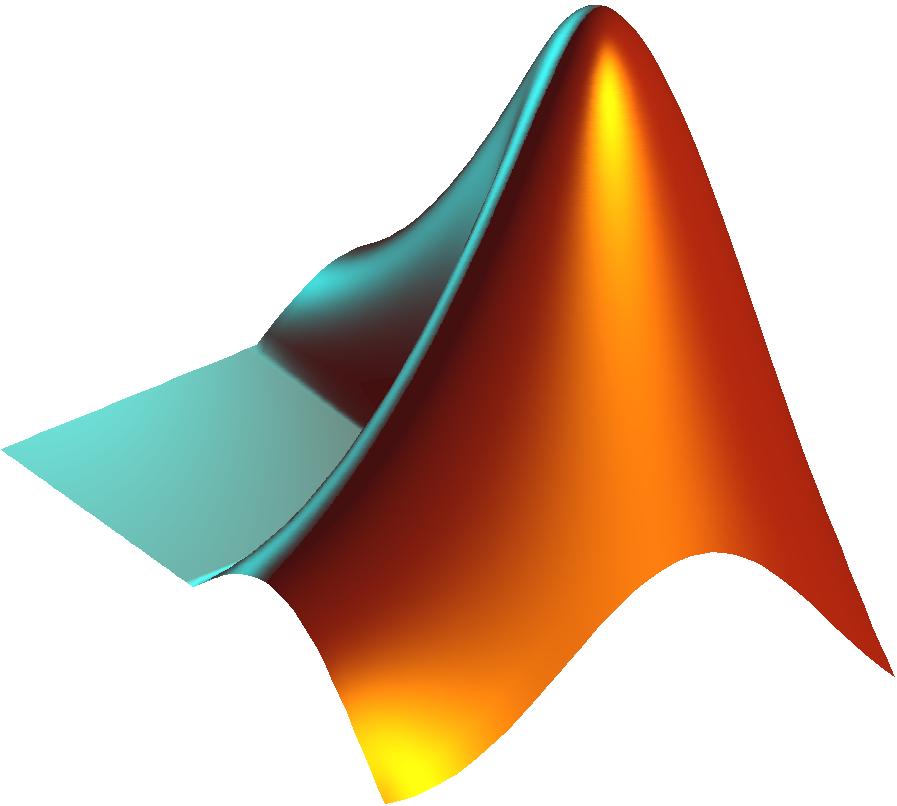
\includegraphics[width=0.25\textwidth]{images/Matlab-logo}
%\centering
%\caption{Το λογότυπο του \en{MATLAB}.}
%\label{img:MATLABlogo}
%\end{figure}

\section{Επιρροή μεταβλητών σε έναν \en{Electron Beam Scanner}}

Ενδιαφέρον παρουσιάζει το πώς διάφορες μεταβλητές επηρεάζουν τα στοιχεία της χαρακτηριστικής έλλειψης που παρουσιάστηκαν.
Συγκεκριμένα, διερευνήθηκε πώς επηρεάζουν τη χαρακτηριστική έλλειψη τα εξής μεγέθη:
\begin{enumerate}
	\item Ένταση της κύριας δέσμης $Q_i$ (ανά παλμό)
	\item Μήκος της κύριας δέσμης $\sigma$
	\item Αρχική θέση ριπής $\rho$ κατά $Y$
	\item Τάση της δέσμης ανίχνευσης $V$
\end{enumerate}

Το εύρος των παραμέτρων που μελετήθηκε φαίνεται στον Πίνακα \ref{tab:simulation-ranges}.

\begin{table}[tph]
\centering
	\begin{tabular}{l c S s}
		\toprule
		Μέγεθος & Σύμβολο & {Αρχική Τιμή} & \multicolumn{1}{c}{Μονάδα Μέτρησης}\\		
		\midrule
		Ένταση της κύριας δέσμης	& $Q_i$		& 5.9e-4	& \coulomb \\
		Μήκος της κύριας δέσμης 	& $\sigma$	& 4e-3		& \meter \\
		Αρχική θέση ριπής κατά $Y$ 	& $\rho$	& 1e-2		& \meter \\
		Τάση της δέσμης ανίχνευσης	& $V$		& 2e4		& \volt \\
		\bottomrule
	\end{tabular}
\caption{Οι αρχικές τιμές των παραμέτρων που μελετήθηκαν.}
\label{tab:simulation-initial-values}
\end{table}

\begin{table}[tph]
\centering
	\begin{tabular}{c SS s}
		\toprule
		Σύμβολο & \multicolumn{2}{c}{Εύρος τιμών} & \multicolumn{1}{c}{Μονάδα Μέτρησης}\\	
		\cmidrule{2-3}	
		 & {Ελάχιστη} & {Μέγιστη} & \\
		\midrule
		$Q_i$		& 5.9e-5	& 5.9e-3	& \coulomb \\
		$\sigma$	& 1e-4		& 2e-1		& \meter \\
		$\rho$		& 0			& 2			& \meter \\
		$V$			& 2e2		& 2e6		& \volt \\
		\bottomrule
	\end{tabular}
\caption{Το εύρος των παραμέτρων που μελετήθηκαν στην μελέτη επιρροής μεταβλητών.}
\label{tab:simulation-ranges}
\end{table}

\subsection{Μελέτη θεωρητικού μοντέλου με το \en{MATLAB}} \label{sub:variable-analysis-MATLAB}
Για τη διερεύνηση αυτή δημιουργήθηκε ένα \en{script} στο \en{MATLAB}, όπου χρησιμοποιήθηκε το μοντέλο που παρουσιάστηκε στην υπο-ενότητα \ref{sub:EBS-model} και έγιναν οι μελέτες για το πώς επηρεάζει η κάθε παράμετρος ξεχωριστά τη χαρακτηριστική έλλειψη της δέσμης. 

Για τη διευκόλυνση του αναγνώστη παρατίθενται οι Εξισώσεις \ref{eq:thetayLogatchov1999} και \ref{eq:thetazLogatchov1999} εκ νέου:
\begin{equation}
\theta_y (x) = \frac{2 \rho r_e}{\beta} \int_{-\infty}^{\infty}\frac{n(z) \dd z}{\rho^2 + \left(x+\beta z \right) ^2} \tag{\ref{eq:thetayLogatchov1999}} 
\end{equation}
\begin{equation}
\theta_z(x) = 2 r_e \int_{-\infty}^{\infty}\frac{(x+\beta z)n(z) \dd z}{\rho^2 + \left(x+\beta z \right) ^2}	\tag{\ref{eq:thetazLogatchov1999}} 
\end{equation}

όπου:
\begin{itemize}
\item $r_e$: η κλασική ακτίνα του ηλεκτρονίου
\item $\beta =\frac{v_t}{c}$: η σχετική ταχύτητα της δέσμης ανίχνευσης
\item $c$: η ταχύτητα του φωτός
\item $x$: η θέση σωματιδίου της δέσμης ανίχνευσης τη χρονική στιγμή $t=0$
\item $n(z)$: η γραμμική πυκνότητα της κύριας δέσμης κατά τον άξονα $Z$
\end{itemize} 

Για το σκοπό της ανάλυσης δημιουργήθηκε η συνάρτηση \src{staticBeamDeflection.m} στο \en{MATLAB}, η οποία δέχεται ως ορίσματα τη θέση $x$ του σωματιδίου την $t = 0$, την αρχική θέση ρίψης $\rho$, τη σχετική ταχύτητα $\beta$ της δέσμης ανίχνευσης, τη συνάρτηση γραμμικής πυκνότητας $n(z)$ και το μήκος $\sigma$ της δέσμης, και δίνει ως έξοδο τις γωνίες απόκλισης $\theta_y$ και $\theta_z$, σύμφωνα με τις εξισώσεις Εξισώσεις \ref{eq:thetayLogatchov1999} και \ref{eq:thetazLogatchov1999}.
Η συνάρτηση αυτή παρουσιάζεται στον Κώδικα \ref{lst:staticBeamDeflection}.

Λόγω του γεγονότος ότι το παραπάνω μοντέλο δε έχει ως μεταβλητές κάποιες από αυτές που θέλουμε να μελετήσουμε ως έχουν χρειάστηκε να γίνουν κάποιες μετατροπές. 
Συγκεκριμένα για την ένταση της κύριας δέσμης και την τάση της δέσμης ανίχνευσης, χρησιμοποιήσαμε τις παρακάτω ιδιότητες:

\begin{itemize}
	\item Η ένταση της κύριας δέσμης $Q_i$ ανά παλμό επηρεάζει τα ηλεκτρόνια ανά δέσμη $N_e$ σύμφωνα με την εξίσωση $N_e = \frac{Q_i}{N_b q_e}$, όπου $N_b$ ο αριθμός δεσμών ανά παλμό και $q_e$ το στοιχειώδες φορτίο του ηλεκτρονίου.
	Επομένως, έτσι επηρεάζεται η γραμμική πυκνότητα της κύριας δέσμης $n(z)$ κατά τον άξονα $Z$ ως εξής: $n(z) = N_e \cdot \mathcal{N}\left(0, \sigma^2 \right)$.
	\item Η τάση της δέσμης ανίχνευσης $V$ επηρεάζει τον παράγοντα \en{Lorenz} $\gamma = 1 + \frac{V}{E_0}$, όπου για το $\gamma$ ισχύει ότι η ενέργεια $E$ κινούμενου σωματιδίου ισούται με $E = \gamma E_0 = \gamma m_ 0c^2$. 
	Έτσι, επηρεάζεται η σχετική ταχύτητα $\beta =\frac{v_t}{c}$ της δέσμης ανίχνευσης, λόγω του ότι $\beta = \sqrt{1 - \frac{1}{\gamma^2}}$ \cite{Forshaw2014}.
\end{itemize}

\lstinputlisting[
	float,
	language=matlab, 
	label={lst:staticBeamDeflection}, 
	caption={\tg{Η συνάρτηση υπολογισμού των γωνιών απόκλισης της δέσμης}.}]
{code/EBS-variable-analysis/staticBeamDeflection.m}

\subsection{Μελέτη επιρροής μεταβλητών με το \en{CST}} \label{sub:variable-analysis-CST}
Η ίδια μελέτη έγινε και στο \en{CST}, με σκοπό να φανεί το πώς επηρεάζουν οι μεταβλητές αυτές το μοντέλο, όταν αυτό προσομοιωθεί ως κατασκευή.

Τα μεγέθη που μεταβλήθηκαν για την εξαγωγή των αποτελεσμάτων φαίνονται στον Πίνακα \ref{tab:CST-variables-corresponding}. 
%Η μόνη διαφοροποίηση σχετικά με τον τρόπο που έγινε η προσομοίωση στο \en{CST} αφορά την τάση $V$ της δέσμης ανίχνευσης. 
%Καθώς αυτό το μέγεθος δε χρησιμοποιείται έτσι στο μοντέλο του \en{CST}, αυτό έπρεπε να μετατραπεί σε ενέργεια της δέσμης ανίχνευσης. 
%Αυτό έγινε ως εξής:
%\begin{equation}
%\begin{split}
%E &= \gamma E_0 = \left(1 + \frac{V}{E_0} \right) E_0 = E_0 + V = m_0 c^2 + V = N_e m_e c^2 + V  = \frac{Q_i}{N_b q_e}m_e c^2 + V \\
%&= \frac{5.9 \times 10^{-4}}{70128 q_e}m_e c^2 + V = \\
%&\Longrightarrow   
%\begin{cases}
%    E_{min} = 2,    & \quad V = V_{min} = \text{\SI{2e2}{\volt}}\\
%    E_{max} = 3,	& \quad V = V_{max} = \text{\SI{2e6}{\volt}}
%  \end{cases}
%\end{split}   
%\end{equation}

\begin{table}[tph]
\centering
	\begin{tabular}{l c l}
		\toprule
		Μέγεθος & Σύμβολο & Παράμετρος του μοντέλου \en{CST}\\		
		\midrule
		Ένταση της κύριας δέσμης	& $Q_i$		& \src{main\_beam\_charge} \\
		Μήκος της κύριας δέσμης 	& $\sigma$	& \src{main\_beam\_length}\\
		Αρχική θέση ριπής κατά $Y$ 	& $\rho$	& \src{scan\_beam\_vertical\_offset}\\
		Τάση της δέσμης ανίχνευσης	& $V$		& \src{scan\_beam\_energy}\\
		\bottomrule
	\end{tabular}
\caption{Αντιστοιχία των μεταβλητών που μελετήθηκαν με το αντίστοιχο μέγεθος στο μοντέλο του \en{CST}.}
\label{tab:CST-variables-corresponding}
\end{table}

\section{Προσομοίωση \en{Electron Beam Scanner} στο \en{CST}} \label{sec:EBS-in-CST}

\subsection{Περιγραφή του μοντέλου}
Στη συνέχεια ξεκίνησε η δημιουργία του \en{CST model} που θα υπολογίζει το ακριβές προφίλ της δέσμης, δηλαδή η πλήρης προσομοίωση ενός \en{Electron Beam Scanner}.

Το μοντέλο περιλαμβάνει τους δύο σωλήνες ίδιας διαμέτρου, της κύριας δέσμης και της δέσμης ανίχνευσης, οι οποίοι τέμνονται κάθετα με κέντρο την αρχή των αξόνων. Οι σωλήνες είναι από κενό και βρίσκονται μέσα σε χώρο τέλειου αγωγού (\en{Perfect Electric Conductor, PEC}).
Στην αρχή του κάθε σωλήνα βρίσκεται από μια πηγή σωματιδίων, (\en{Particle Source}). 
Η κύρια δέσμη εκπέμπει 10 δέσμες σωματιδίων με \en{Gaussian emission model}, ενώ η δέσμη ανίχνευσης εκπέμπει συνεχόμενα με μοντέλο \en{DC}. 
Το μοντέλο απεικονίζεται στο Σχήμα \ref{fig:CST-PICmonitor} και η πηγή σωματιδίων της κύριας δέσμης στο Σχήμα \ref{fig:CST-mainBeamSource}.

Για την ευκολότερη επαλήθευση της ακρίβειας των αποτελεσμάτων του \en{Electron Beam Scanner}, προστέθηκε ένας \en{PIC Position Monitor} σε όλη την κατασκευή, κάτι που μας επιτρέπει να γνωρίζουμε ανά πάσα χρονική στιγμή τις θέσεις στις οποίες έχουμε σωματίδια.
Ακόμη, προστέθηκαν δύο \en{PIC 2D Monitors}, τα οποία ανιχνεύουν τη διέλευση σωματιδίων στο επίπεδο που βρίσκονται.
Το ένα τοποθετήθηκε στην κύρια δέσμη, λίγο πριν την αλληλεπίδρασή της με τη δέσμη ανίχνευσης, ενώ το δεύτερο τοποθετήθηκε στο τέλος της δέσμης ανίχνευσης.
Το τελευταίο αποτελεί και το $``$αποτέλεσμα$"$ του \en{Electron Beam Scanner}, από το οποίο υπολογίζεται και το προφίλ της δέσμης που ανιχνεύουμε.

Στο \en{CST project} όλες οι διαστάσεις και τα μεγέθη εισάγονται ως παράμετροι, οι οποίες μπορούν να τροποποιηθούν. Οι τελικές παράμετροι του μοντέλου που χρησιμοποιήθηκε παρατίθενται στο Παράρτημα \ref{ch:CSTmodel}, στην ενότητα \ref{sec:CSTparameterlist}.

\begin{figure}[tbh]
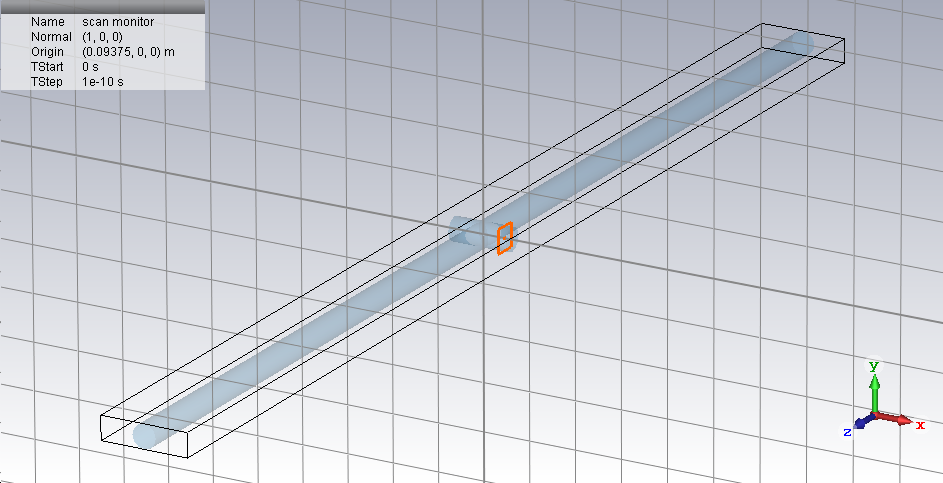
\includegraphics[width=\textwidth]{figures/CST-pic-monitor}
\centering
\caption[Η διάταξη προσομοιωμένη στο \en{CST}.]
{Η διάταξη προσομοιωμένη στο \en{CST}. 
Στον σωλήνα της δέσμης ανίχνευσης φαίνεται ανιχνευτής σωματιδίων (\en{PIC 2D monitor}), όπου ανιχνεύονται η απόκλιση της δέσμης ανίχνευσης και με βάση αυτό εκτιμάται το προφίλ της κύριας δέσμης.}
\label{fig:CST-PICmonitor}
\end{figure}

\begin{figure}[tbh]
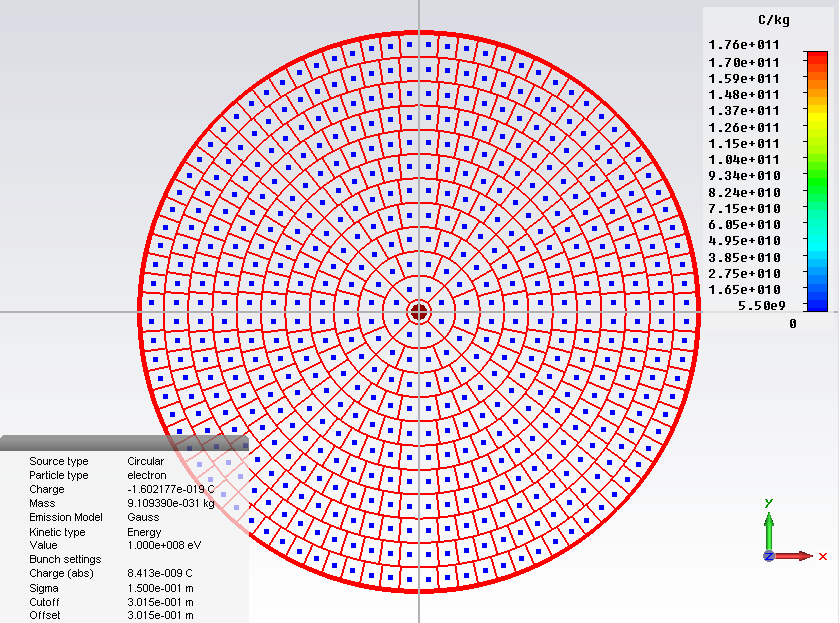
\includegraphics[width=\textwidth]{figures/CST-main-beam-source}
\centering
\caption[Η πηγή της κύριας δέσμης στο \en{CST}.]
{Η πηγή της κύριας δέσμης στο \en{CST}. 
Με μπλε χρώμα φαίνονται τα $``$\en{emission points}$"$, τα σημεία απ' όπου εκπέμπονται ηλεκτρόνια.}
\label{fig:CST-mainBeamSource}
\end{figure}


\subsection{Υπολογισμός αποτελεσμάτων}

Ο υπολογισμός των αποτελεσμάτων γίνεται αποκλειστικά μέσα στο \en{CST}, μέσω \en{Template Based Post Processing}.

Συγκεκριμένα, υπολογίζονται 26 αποτελέσματα:
\begin{itemize}

\item Η μέση τιμή των συντεταγμένων $x$, $y$ και $z$ των σωματιδίων που φτάνουν στον \en{PIC 2D Monitor}, δηλαδή στο πέτασμα του \en{Electron Beam Scanner}, την κάθε χρονική στιγμή.

\item Οι γωνίες απόκλισης $\theta_y$ και $\theta_z$, υπολογίζοντας το τόξο της γωνίας με εφαπτομένη το λόγο της διαφοράς της θέσης στον αντίστοιχο άξονα από την ριπή της δέσμης μέχρι την άφιξη στον \en{PIC 2D Monitor} προς την απόσταση του σημείου ριπής και ανίχνευσης. 
Δηλαδή $\theta_y = \tan^{-1} \left( \frac{\bar{y} - \rho}{\Delta x} \right)$ και αντίστοιχα $\theta_z = \tan^{-1} \left( \frac{\bar{z} - 0}{\Delta x} \right)$, αφού κατά τον άξονα $Z$ η αρχική θέση είναι η $z = 0$. 
Οι γωνίες υπολογίζονται και προβάλλονται σε κοινή γραφική παράσταση συνολικά και για τις 10 δέσμες, αλλά και για την 1\textsuperscript{η} και 10\textsuperscript{η} δέσμη ξεχωριστά.

\item Οι μέγιστες και ελάχιστες τιμές των $\theta_y$ και $\theta_z$ συνολικά για όλες τις δέσμες μιας προσομοίωσης, αλλά και για την 1\textsuperscript{η} και 10\textsuperscript{η} δέσμη της προσομοίωσης ξεχωριστά.

\item Το ύψος, το πλάτος και τον λόγο της χαρακτηριστικής έλλειψη της δέσμης. Το ύψος ισούται με τη $\theta_{y, \text{\en{max}}}$, το πλάτος με $\theta_{z, \text{\en{max}}} - \theta_{z, \text{\en{min}}}$ και ο λόγος με το ύψος προς το πλάτος της χαρακτηριστικής έλλειψης.

\item Η γραφική παράσταση της χαρακτηριστικής έλλειψης της δέσμης, συνδυάζοντας τις μεταβλητές $\theta_y$ και $\theta_z$ στους άξονες $Y$ και $X$ αντίστοιχα. 
Απεικονίζονται οι ελλείψεις όλων των δεσμών μαζί, καθώς και η έλλειψη της 1\textsuperscript{ης} δέσμης ξεχωριστά.

\item Τέλος, υπολογίζεται η παράγωγος των μεγίστων των $\theta_y$, όταν αυτή έχει υπολογιστεί μέσω \en{parameter sweep} για εύρος αρχικών θέσεων ρίψης $\rho$, ως προς το $\rho$, το οποίο μας δίνει την τελική εκτίμηση του προφίλ της δέσμης από την κατασκευή μας, όπως περιγράφεται στην Εξίσωση \ref{eq:transverseProfile}.

\end{itemize}

\begin{figure}[tph]
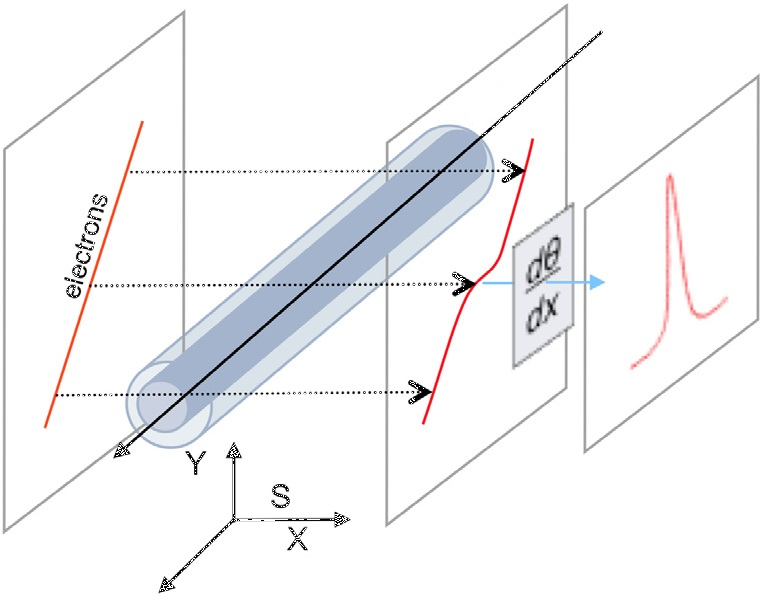
\includegraphics[width=0.6\textwidth]{figures/EBS-profile-calculation}
\centering
\caption{Γραφική παρουσίαση του τρόπου εκτίμησης του προφίλ δέσμης με \en{Electron Beam Scanner} \cite{Blokland2009}.}
\label{fig:EBS-profile-calculation}
\end{figure}

Το τελικό μοντέλο προέκυψε ύστερα από πολλά στάδια δοκιμών για την ακρίβεια αποτελεσμάτων και βελτιστοποιήσεων χρονικής απόδοσης.
Η αναλυτική περιγραφή όλων των μεθόδων \en{post processing} που χρησιμοποιήθηκαν στο μοντέλο στο \en{CST} βρίσκεται στην ενότητα \ref{sec:CSTpostProcessing} του Παραρτήματος \ref{ch:CSTmodel}.

\begin{figure}[tbh]
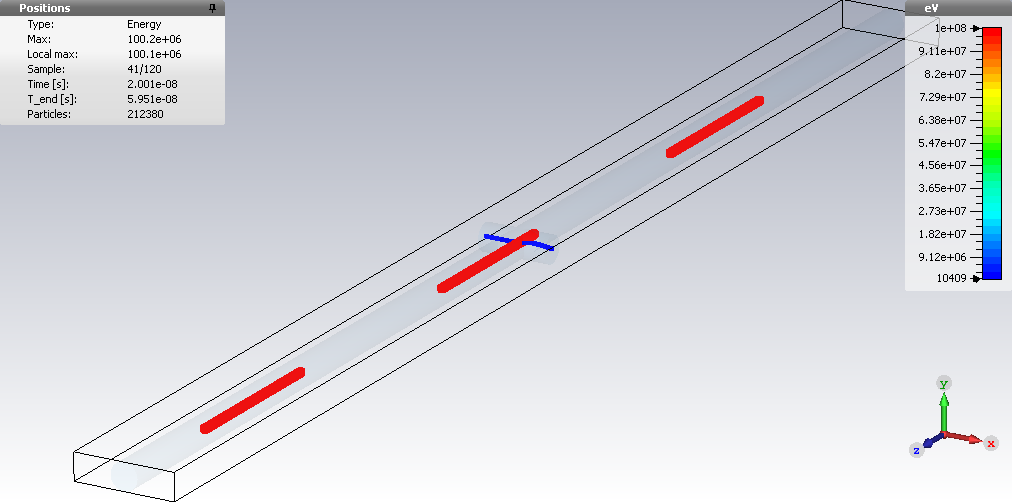
\includegraphics[width=\textwidth]{figures/CST-EBS-implementation/CST-multi-bunch-EBS-detection}
\centering
\caption[Η διαδικασία ανίχνευσης του προφίλ της δέσμης από τον \en{Electron Beam Scanner} στο \en{CST}.]
{Η διαδικασία ανίχνευσης του προφίλ της δέσμης από τον \en{Electron Beam Scanner} στο \en{CST}.
Βλέπουμε την εκτροπή της δέσμης ανίχνευσης (μπλε) από την κύρια δέσμη (κόκκινο) που αλληλεπιδρά με τη δέσμη ανίχνευσης.}
\label{fig:CST-MultiBunchEBSDetection}
\end{figure}

\subsection{Δημιουργία \en{Gaussian} δέσμης στο \en{CST}}

Για τον υπολογισμό του προφίλ μιας \en{Gaussian} δέσμης, συναντήσαμε το πρόβλημα ότι μετά τον υπολογισμό του προφίλ, το σχήμα δε φαινόταν να έχει αυτό που ήταν αναμενόμενο.

\begin{figure}[tph]
	\begin{subfigure}{\textwidth}
		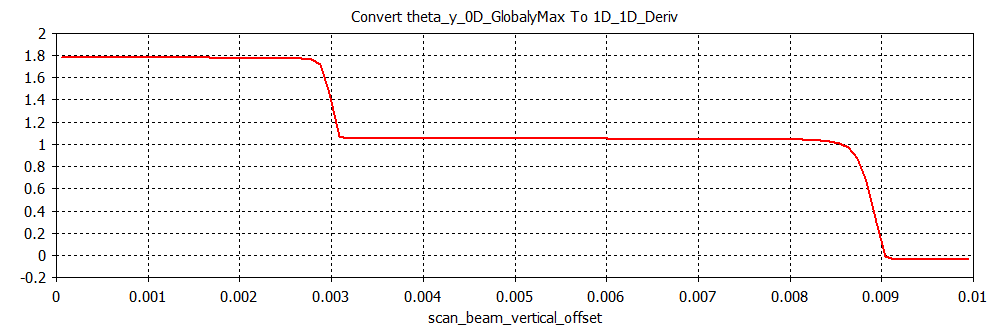
\includegraphics[width=\textwidth]{figures/CST-profile-steps}
		\centering
		\caption{Το αποτέλεσμα του υπολογισμού του προφίλ στο \en{CST} για $c_{\text{\en{off}}} = 2$. 
		Η μορφή του δεν είναι \en{Gaussian}}
		\label{fig:CST-profile-steps}
	\end{subfigure}
	\begin{subfigure}{\textwidth}
		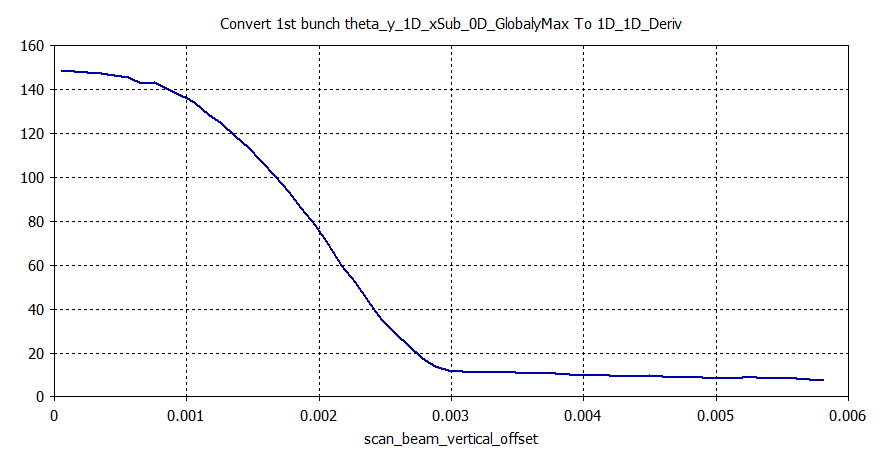
\includegraphics[width=\textwidth]{figures/CST-profile-nosteps}
		\centering
		\caption{Το αποτέλεσμα του υπολογισμού του προφίλ στο \en{CST} για $c_{\text{\en{off}}} = 8.0027$ έχει \en{Gaussian} μορφή.}
		\label{fig:CST-profile-nosteps}
	\end{subfigure}
\caption{Σύγκριση του αποτελέσματος υπολογισμού του προφίλ της δέσμης για $c_{\text{\en{off}}} = 2$ και $c_{\text{\en{off}}} = 8.0027$.}
\label{fig:CST-profile-stepcomparison}
\end{figure}

Για την επίλυση του προβλήματος αυτού, αρχικά ελέγξαμε αν το πρόβλημα βρίσκεται στον τρόπο δημιουργίας της δέσμης ή στον τρόπο ανίχνευσης. 
Έτσι:
\begin{enumerate}
\item Δημιουργήσαμε ένα νέο \en{CST project} και, αφού στήθηκε όλο το μοντέλο εκ νέου, μπήκε ένας \en{particle monitor} που ανιχνεύει τα σωματίδια της κύριας δέσμης.
\item Έγινε εξαγωγή των δεδομένων αυτών της κύριας δέσμης.
\item Τα δεδομένα αυτά εισήχθησαν στο \en{MATLAB} και δημιουργήθηκε το κατάλληλο \en{script} για την ανάλυσή τους.
\end{enumerate}

Από την παραπάνω διαδικασία έγινε σαφές ότι το πρόβλημα εντοπίζεται στον τρόπο που το \en{CST} δημιουργεί την κατανομή των σωματιδίων.

\subsection{Τρόπος δημιουργίας \en{Gaussian} κατανομών σωματιδίων στο \en{CST}}

Μετά από αναζήτηση και επικοινωνία με το ίδιο το \en{support} του \en{CST}, έγινε σαφής ο τρόπος που γίνεται η προσομοίωση των σωματιδίων για \en{Gaussian} κυκλικές πηγές σωματιδίων.
%TODO citation needed
Συγκεκριμένα, αρχικά, αφού το συνολικό ποσό φορτίου που εκπέμπεται δεν μεταβάλλεται ανάλογα με τη συνάρτηση κατανομής τίθεται ο περιορισμός ότι:
\begin{equation}\label{eq:CST-gaussian-restriction}
2\pi \int_{R_{\text{\en{in}}}}^{R_{\text{\en{out}}}} f(r) \dd r = \pi \left(R_{\text{\en{out}}}^2 - R_{\text{\en{in}}}^2 \right) 
\end{equation}

όπου:
\begin{itemize}
\item $R_{\text{\en{out}}}$: η εξωτερική ακτίνα της κυκλικής πηγής σωματιδίων
\item $R_{\text{\en{in}}}$: η εσωτερική ακτίνα της κυκλικής πηγής σωματιδίων (στην περίπτωσή μας $R_{\text{\en{in}}} = 0$)
\item $f(r)$: η συνάρτηση ακτινικής κατανομής 
\end{itemize} 

Η παραπάνω σχέση χρησιμοποιείται για να κλιμακοποιήσει τη συνάρτηση κατανομής. 
Η λογική του τρόπου υπολογισμού αυτού είναι ότι η συνάρτηση κατανομής θα πρέπει να υπολογίζεται με τρόπο, ώστε ο συνολικός αριθμός του φορτίου που εκπέμπεται να είναι ανεξάρτητος από την ορισμένη κατανομή.
Αυτό σημαίνει ότι ο συντελεστής κατανομής $c_{\text{\en{scale}}}$ υπολογίζεται αυτόματα.

Στη συνέχεια, η \en{Gaussian} κατανομή δίνεται από τη σχέση:
\begin{equation}
f(r) = c_{\text{\en{off}}} + c_{\text{\en{scale}}} \left( \exp \left(-\frac{r^2}{2\sigma^2}\right) - 1 \right)
\end{equation}

όπου:
\begin{itemize}
\item $c_{\text{\en{off}}}$: η τιμή της συνάρτησης για $r = 0$
\item $\sigma$: η τυπική απόκλιση
\end{itemize} 

\begin{figure}[tph]
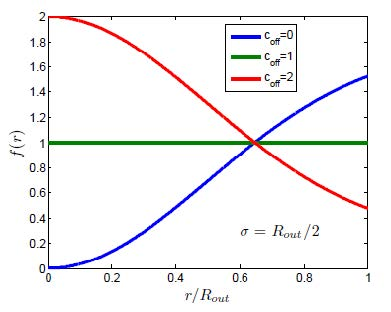
\includegraphics[width=0.6\textwidth]{figures/CST-gauss-function-for-coff}
\centering
\caption{Παράδειγμα \en{Gaussian} συνάρτησης για διάφορες τιμές του συντελεστή $c_{\text{\en{off}}}$.}
\label{fig:CST-gauss-coff}
\end{figure}

Για να έχουμε μια πραγματικά \en{Gaussian} δέσμη, θέλουμε να ισχύει
\[c_{\text{\en{off}}} = 0\]

Αφού οι υπόλοιπες μεταβλητές είναι καθορισμένες από τις απαιτήσεις του επιταχυντή, απομένει να βρεθεί η τιμή του $c_{\text{\en{scale}}}$ που θα μας δίνει τη ζητούμενη συνθήκη.

\subsection{Υπολογισμός του κατάλληλου συντελεστή κλιμακοποίησης για \en{Gaussian} δέσμη}

Ο τρόπος που υπολογίζει το \en{CST} την \en{Gaussian} κατανομή, όπως είδαμε παραπάνω είναι
\begin{eqnarray}\label{eq:CST-gaussian-model}
f(r) &= & 	c_{\text{\en{off}}} + c_{\text{\en{scale}}} \left( \exp \left(-\frac{r^2}{2\sigma^2}\right) - 1 \right) \nonumber \\
&= &\left(c_{\text{\en{off}}} - c_{\text{\en{scale}}}\right) + c_{\text{\en{scale}}} e^{-\frac{r^2}{2\sigma^2}}
\end{eqnarray}

Η πραγματική κατανομή της δέσμης στον επιταχυντή που μελετούμε όμως, έχει γενική μορφή κατανομής:
\begin{equation}\label{eq:General-gaussian-model}
 f(r) = a e^{-\frac{\left(r-b\right)^2}{2c^2}}
\end{equation}

Επομένως, εξισώνοντας τις παραπάνω σχέσεις \ref{eq:CST-gaussian-model} και \ref{eq:General-gaussian-model} και δεδομένου ότι πρέπει να ισχύουν $\forall \; r$ προκύπτουν τα συμπεράσματα ότι:
\begin{eqnarray}
a &\equiv & c_{\text{\en{scale}}}\nonumber \\
b &= &0\nonumber \\
c &\equiv & \sigma \nonumber \\
c_{\text{\en{off}}} &=&  c_{\text{\en{scale}}} 
\end{eqnarray}

Επομένως, πρέπει να βρεθεί ο κατάλληλος συνδυασμός τιμών $\left(c_{\text{\en{off}}}, c_{\text{\en{scale}}}\right)$ που να πληροί τον περιορισμό της εξίσωσης \ref{eq:CST-gaussian-restriction}, δεδομένων των τιμών των μεταβλητών $\sigma, R_{\text{\en{out}}}$ και $R_{\text{\en{in}}}$ του επιταχυντή μας.

Για την επίλυση του παραπάνω προβλήματος δημιουργήθηκε κατάλληλο \en{script} στο \en{MATLAB}. 

Αρχικά δημιουργήθηκε η συνάρτηση \src{cscale = calculateCscale( sigma, coff, Rout, Rin)} η οποία δέχεται ως ορίσματα τις μεταβλητές: $\sigma, c_{\text{\en{off}}}, R_{\text{\en{out}}}$ και $R_{\text{\en{in}}}$ και δίνει στην έξοδό του την τιμή του $c_{\text{\en{scale}}}$ που πληροί την εξίσωση \ref{eq:CST-gaussian-restriction}.

Στη συνέχεια, τρέχοντας το \en{script} \src{findOptimumCoff.m} δίνουμε τις τιμές των παραμέτρων του προβλήματός μας στα $\sigma, c_{\text{\en{off}}}, R_{\text{\en{out}}}, R_{\text{\en{in}}}$ και βρίσκουμε την τιμή του $c_{\text{\en{off}}}$ που επαληθεύει τη σχέση $c_{\text{\en{off}}} = c_{\text{\en{scale}}} \left(\sigma, c_{\text{\en{off}}}, R_{\text{\en{out}}}, R_{\text{\en{in}}} \right)$.

\lstinputlisting[
	float,
	language=matlab, 
	label={lst:calculateCscale}, 
	caption={\tg{Η συνάρτηση υπολογισμού του $c_{\text{\tl{scale}}}$}.}]
{code/calculating-optimum-coff/calculateCscale.m}

\lstinputlisting[
	float,
	language=matlab, 
	label={lst:findOptimumCoff}, 
	caption={\tg{Το }\en{script}\tg{ υπολογισμού του κατάλληλου για τα δεδομένα μας $c_{\text{\tl{off}}}$}.}]
{code/calculating-optimum-coff/findOptimumCoff.m}

Εν τέλει, για τις τιμές του δικού μας προβλήματος, δίνουμε ως είσοδο $\left(\sigma, R_{\text{\en{out}}}, R_{\text{\en{in}}} \right) = \left(0.01/4,0.01, 0 \right)$ και προκύπτει η ζητούμενη τιμή του συντελεστή:
\begin{equation}
	\boxed{c_{\text{\en{off}}} \approx 8.002684}
\end{equation}

Ο υπολογισμός του συντελεστή για διαφορετικές τιμές των $\sigma, R_{\text{\en{out}}}$ και $R_{\text{\en{in}}}$ δεν έχουμε παρά να αλλάξουμε τις τιμές στον Κώδικα \ref{lst:findOptimumCoff} και να τρέξουμε εκ νέου το πρόγραμμα.

\section{Ανάλυση δεσμών στο \en{MATLAB}}

Με σκοπό τη βελτιστοποίηση της ταχύτητας προσομοίωσης, ώστε να είναι δυνατή η προσομοίωση παλμών (\en{pulses}, πολλαπλών δεσμών) και τρένων (\en{trains}, πολλαπλών παλμών) σωματιδίων, η διαδικασία προσομοίωσης επεκτάθηκε και στην ενεργή χρήση του \en{MATLAB}.
Η διαδικασία προσομοίωσης σε αυτή την περίπτωση παίρνει τη μορφή:
\begin{enumerate}
\item Ηλεκτρομαγνητική προσομοίωση του κύριου σωλήνα του επιταχυντή στο \en{CST}, που περιλαμβάνει την κύρια δέσμη, όσες φορές είναι επιθυμητό
\item Εξαγωγή των αποτελεσμάτων της προσομοίωσης από το \en{CST} σε μορφή αρχείου \en{ASCII}
\item Μετατροπή των αποτελεσμάτων της προσομοίωσης σε μορφή αρχείου \en{MATLAB formatted data} (\src{.mat}) για βελτιστοποίηση στο χώρο αποθήκευσης και χρόνο προσπέλασης
\item Εισαγωγή και προεπεξεργασία των δεδομένων στο \en{MATLAB}
\item Υπολογισμός των τροχιών σωματιδίων της δέσμης ανίχνευσης μέσα από το \en{MATLAB} στο προσομοιωμένο μαγνητικό πεδίο
\end{enumerate}

\subsection{Προσομοίωση του κύριου σωλήνα του επιταχυντή στο \en{CST}}
Για την προσομοίωση του κύριου σωλήνα δημιουργήθηκε ένα νέο \en{project} στο \en{CST}.
Το \en{project} αυτό περιέχει τη γεωμετρία που χρησιμοποιήθηκε και στο \en{project} με τις δύο δέσμες, δηλαδή δύο κάθετοι σωλήνες ίδιας διαμέτρου που περιλαμβάνουν κενό, μέσα σε χώρο τέλειου αγωγού (\en{PEC}).
Αυτή τη φορά έχουμε μόνο ένα \en{Particle Source}, την κύρια δέσμη, που εκπέμπει σωματίδια με \en{Gaussian emission model}.

Γύρω από το χώρο διασταύρωσης των σωλήνων της κύριας δέσμης και της δέσμης ανίχνευσης έχει τοποθετηθεί ένας \en{E-field monitor}, που αποθηκεύει τις τιμές του ηλεκτρικού πεδίου σε κάθε χρονική στιγμή της προσομοίωσης. 
Οι τιμές αυτές είναι αυτές που θα εξαχθούν για να χρησιμοποιηθούν στα επόμενα βήματα.

Η διάταξη φαίνεται στο Σχήμα \ref{fig:CST-export-main-beam-project-efield-box}.

\begin{figure}[tbh]
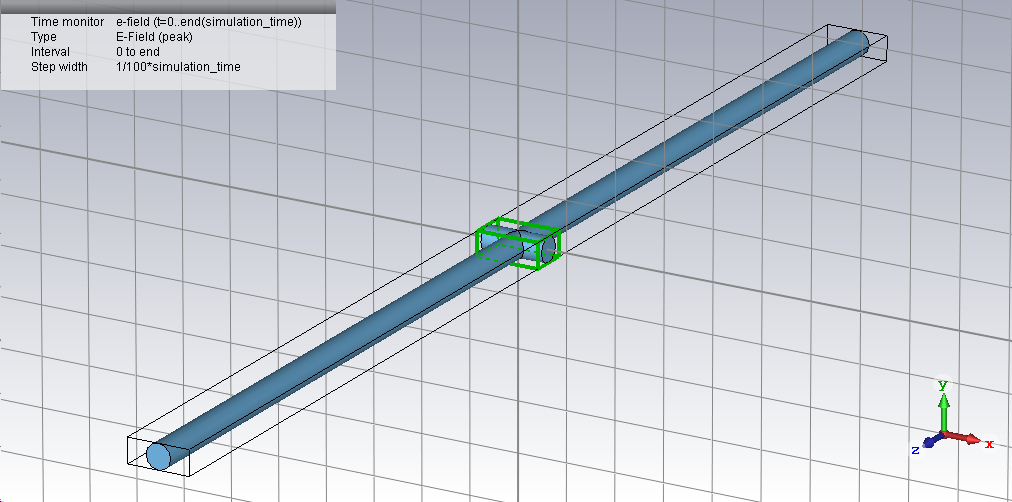
\includegraphics[width=\textwidth]{figures/export-main-beam-project-efield-box}
%from Project v0.51 reworked with export.cst
\centering
\caption[Η διάταξη προσομοίωσης του κύριου σωλήνα στο \en{CST}.]
{Η διάταξη προσομοίωσης του κύριου σωλήνα στο \en{CST}.
Με πράσινο χρώμα φαίνεται ο \en{E-field monitor}.}
\label{fig:CST-export-main-beam-project-efield-box}
\end{figure}

\subsection{Εξαγωγή των αποτελεσμάτων του \en{CST}}
Μετά την εκτέλεση της προσομοίωσης, τα αποτελέσματα εξάγονται από το πρόγραμμα, επιλέγοντας τα αποτελέσματα στο φάκελο \en{e-field}, μέσα στα \en{2D/3D Results} και κάνοντας \en{export} από την καρτέλα \en{Post Processing} στη μορφή \en{ASCII}.

Έτσι, τα αποτελέσματα εξάγονται σε μορφή \src{.txt}, που έχει 9 στήλες: 3 στήλες για τη θέση κάθε σωματιδίου (συντεταγμένες $x$, $y$ και $z$) και 6 για τις τιμές του ηλεκτρικού πεδίου στη θέση αυτή ($\operatorname{Re}(E_x)$, $\operatorname{Re}(E_y)$, $\operatorname{Re}(E_z)$, $\operatorname{Im}(E_x)$, $\operatorname{Im}(E_y)$, $\operatorname{Im}(E_z)$).
Τα αποτελέσματα απεικονίζουν όλες τις παραπάνω τιμές ξεκινώντας από το πρώτο \en{sample} και συνεχίζοντας μέχρι το τελευταίο.
Στον Κώδικα \ref{lst:CSTasciiOutput} φαίνεται ένα δείγμα εξόδου.

\lstinputlisting[
	float,
	label={lst:CSTasciiOutput}, 
	caption={\tg{Δείγμα εξόδου ενός }\en{e-field monitor }\tg{του}\en{ CST }\tg{σε μορφή }\en{ASCII}.},
	language={},
	backgroundcolor=\color{white},
	basicstyle=\tiny\ttfamily\selectlanguage{english},
	frame=none,
    numbers=none,                        
    tabsize=2,	
    literate={\ \ \ }{{\ \ }}2 {---}{{--}}2,]
{code/CST-output/CST-efieldmonitor-ascii-output.txt}

\subsection{Μετατροπή των αποτελεσμάτων}

Τα αποτελέσματα, όπως βγαίνουν από το \en{CST}, είναι σε μορφή εύκολη για ανάγνωση από άνθρωπο αλλά όχι για επεξεργασία ή αποτελεσματική αποθήκευση. 
Για το λόγο αυτό, τα αποτελέσματα μετατρέπονται σε άλλη μορφή. 

Η μορφή που επιλέχθηκε για τη μετατροπή των δεδομένων είναι η μορφή αρχείου \en{MATLAB formatted data} (\src{.mat}).
Η επιλογή έγινε με βάση την απόδοση του τύπου αρχείου σε χώρο αποθήκευσης και χρόνο προσπέλασης, καθώς και το γεγονός ότι χρησιμοποιείται το \en{MATLAB} για την χρήση των δεδομένων στα επόμενα στάδια της διαδικασίας.

Για τη μετατροπή αυτή δημιουργήθηκε η συνάρτηση \src{importField.m}, η οποία ουσιαστικά είναι \en{parser} αρχείων της μορφής που παρουσιάστηκε, και τα αποθηκεύει σε έναν πίνακα της μορφής $\text{\en{Field}} = \text{\en{Samples}} \times \text{Μεταβλητές} \times \text{Τιμές}$.
Η συνάρτηση ανοίγει το αρχείο των αποτελεσμάτων του \en{CST} και το διαβάζει γραμμή-γραμμή αγνοώντας τις πρώτες 2 γραμμές. 
Αν η γραμμή περιέχει δεδομένα, τα αποθηκεύει στον πίνακα, στο τρέχον \en{Sample}, αλλιώς (αν δηλαδή περιέχει το \en{string } \src{Sample X}) αυξάνει το τρέχον \en{Sample} κατά 1. 
Κατά τη διαδικασία αυτή αγνοούμε τις 3 τελευταίες στήλες, που περιέχουν τα δεδομένα $\operatorname{Im}(E_x)$, $\operatorname{Im}(E_y)$ και $\operatorname{Im}(E_z)$, καθώς για την περίπτωσή μας δεν έχουμε μιγαδική συνιστώσα στο ηλεκτρικό πεδίο.
Τμήμα του κώδικα φαίνεται στον Κώδικα \ref{lst:importField}. 
Δεν παρατίθεται το κομμάτι που αρχικοποιεί τις διαστάσεις του πίνακα.

\lstinputlisting[
	float,
	language=matlab, 
	label={lst:importField}, 
	linerange={1-8, 44-62}, 
	caption={\tg{Τμήμα της συνάρτησης }\src{importField.m}.}]
{code/particle-path-calculation/importField.m}

\subsection{Εισαγωγή και προεπεξεργασία των δεδομένων στο \en{MATLAB}}

Αφού γίνει η μετατροπή του αρχείου σε επεξεργάσιμη μορφή, τα δεδομένα εισάγονται στο \en{MATLAB} για επεξεργασία και χρήση.
Η μορφή πίνακα, στην οποία είναι αποθηκευμένα, αν και πιο βολική από την αρχική, χρειάζεται επιπλέον επεξεργασία για την αποτελεσματική χρήση των δεδομένων.
Συγκεκριμένα, για να υπολογιστεί η τροχιά σωματιδίων στο ηλεκτρικό πεδίο που λαμβάνουμε από το \en{CST}, θα χρειαστεί να κάνουμε παρεμβολή για τη θέση του σωματιδίου σε κάθε χρονική στιγμή, για να βρούμε την τιμή του πεδίου στη θέση αυτή και να υπολογίσουμε την επόμενη. 
Η παρεμβολή αυτή απαιτεί τα δεδομένα να βρίσκονται σε μορφή \en{mesh}.

Έτσι, μετατρέπουμε τον πίνακα που λαμβάνουμε από το προηγούμενο πίνακα σε ένα $``$\en{cell array}$"$ που περιέχει ως στοιχεία πίνακες σε \en{mesh format}, έναν για κάθε χρονική στιγμή. 
Αυτή η διαδικασία πραγματοποιείται με τη συνάρτηση \src{convertFieldDataToCell.m}

Τμήμα του κώδικα της συνάρτησης φαίνεται στον Κώδικα \ref{lst:convertFieldDataToCell}. 
Δεν παρατίθεται το κομμάτι που κάνει αλλαγές στη σειρά αποθήκευσης των μεταβλητών μέσα στο \en{cell}.

\lstinputlisting[
	float,
	language=matlab, 
	label={lst:convertFieldDataToCell}, 
	linerange={1-9,16-37, 51-60}, 
	caption={\tg{Τμήμα της συνάρτησης }\src{convertFieldDataToCell.m}.}]
{code/particle-path-calculation/convertFieldDataToCell.m}

\subsection{Υπολογισμός των τροχιών της δέσμης ανίχνευσης}

Στην τελευταία φάση της διαδικασίας υπολογίζουμε τις τροχιές της δέσμης ανίχνευσης.
Η διαδικασία που ακολουθείται είναι η εξής: ξεκινώντας από την πρώτη χρονική στιγμή, δημιουργούμε ένα σωματίδιο κάθε χρονική στιγμή στη θέση αφετηρίας της δέσμης ανίχνευσης, με δεδομένη αρχική ταχύτητα.
Στη συνέχεια, υπολογίζουμε για καθένα από τα σωματίδια το διάνυσμα $\left(x, y, z; v_x, v_y, v_z\right)$, δεδομένης της τιμής  του πεδίου στη θέση που βρίσκεται το σωματίδιο.
Σε περίπτωση που το ηλεκτρικό πεδίο δεν είναι καθορισμένο στη συγκεκριμένη θέση, γίνεται γραμμική παρεμβολή για τον υπολογισμό της τιμής του, κάνοντας χρήση της συνάρτησης του \en{MATLAB} \src{interp3}.

Για την υλοποίηση της διαδικασίας αυτής υλοποιήθηκαν 4 συναρτήσεις.

Για τον υπολογισμό του διανύσματος $\left(x, y, z; v_x, v_y, v_z\right)$ στην επόμενη θέση, δημιουργήθηκε η συνάρτηση \src{calcNextPosition.m}.
Αυτή υπολογίζει τη νέα θέση σύμφωνα με την εξίσωση 

\begin{equation}
\vec{s}_{\text{\en{new}}} = \vec{s}_{\text{\en{old}}} + \vec{v}_{\text{\en{old}}}\, \Delta t
\end{equation}

και στη συνέχεια, αφού υπολογιστεί η τιμή του μαγνητικού πεδίου $\vec{E}_{\text{\en{new}}}$ στη νέα θέση, υπολογίζεται η νέα ταχύτητα με βάση την εξίσωση 
\begin{equation}
	\vec{v}_{\text{\en{new}}} = \vec{v}_{\text{\en{old}}} + \vec{E}_{\text{\en{new}}} \frac{q_e \, \Delta t}{m_e}
\end{equation}
%TODO check if the science is right
Η συνάρτηση \src{calcNextPosition.m} φαίνεται στον Κώδικα \ref{lst:calcNextPosition}.

\lstinputlisting[
	float,
	language=matlab, 	
	label={lst:calcNextPosition}, 
	linerange={1-13,18-29}, 
	caption={\tg{Η συνάρτηση }\src{calcNextPosition.m}.}]
{code/particle-path-calculation/calcNextPosition.m}

Για τον υπολογισμό της τιμής του μαγνητικού πεδίου $\vec{E}_{\text{\en{new}}}$ σε δεδομένη θέση, δημιουργήθηκε η συνάρτηση  \src{calcField.m}, η οποία πραγματοποιεί τη γραμμική παρεμβολή που αναφέρθηκε παραπάνω. 
Η συνάρτηση \src{calcField.m} φαίνεται στον Κώδικα \ref{lst:calcField}.

\lstinputlisting[
	float,
	language=matlab, 
	label={lst:calcField},  
	linerange={1-4,7-27}, 
	caption={\tg{Η συνάρτηση }\src{calcField.m}.}]
{code/particle-path-calculation/calcField.m}

Η υλοποίηση της μεθόδου γίνεται στο σχετικό \src{script}, τμήμα του οποίου παρατίθεται στον Κώδικα \ref{lst:particle-path-calculation-script}.


\lstinputlisting[
	float,
	language=matlab, 
	label={lst:particle-path-calculation-script}, 
	linerange={54-71,96-116}, 
	caption={\tg{Τμήμα του }\en{script}\tg{ που εκτελεί τον υπολογισμό της τροχιάς για ένα σωματίδιο.}}]
{code/particle-path-calculation/script.m}

%not worth mentioning
%\lstinputlisting[language=matlab, float, label={lst:lininterp1}, caption={\tg{Η συνάρτηση }\src{lininterp1.m}}]{code/particle-path-calculation/lininterp1.m}